\documentclass[11pt]{article}
\usepackage[a4paper,margin=1in]{geometry}
\usepackage{amsmath,amssymb,amsthm,mathtools}
\usepackage{graphicx}
\usepackage{hyperref}
\usepackage[section]{placeins}

\title{Mass Shell Perfect Closure: Closed Quaternionic Light and Relativistic Norm Structure}
\author{John Van Geem / RQM Technologies}
\date{April 2026}

\begin{document}
\maketitle

\begin{abstract}
We reformulate the relativistic mass shell in conjugate-norm language suitable for the Perfect Closure program. Starting from $E^2=p^2c^2+m^2c^4$, we define a biquaternionic momentum variable $P=E/c+I\mathbf p$ and show that $P\bar P=m^2c^2$ is exactly the invariant mass-shell statement. We distinguish null/open propagation ($P\bar P=0$) from massive/closed propagation ($P\bar P>0$). We then define Compton curvature $k_C=mc/\hbar$ as the bridge variable for Paper 4. This paper does not derive Standard Model masses.
\end{abstract}

\noindent\textbf{Keywords:} mass shell; relativistic invariant; biquaternions; conjugate norm; Compton curvature; perfect closure.

\section{Introduction}
Paper 3 provides the physical norm target used by the later operator bridge. The objective is conservative: re-express standard relativistic invariants in a closure-compatible algebra without altering their content.

\section{Contributions}
\begin{enumerate}
  \item We restate the standard relativistic mass shell and preserve invariant content.
  \item We show that $P\bar P$ is a conjugate norm statement equivalent to the scalar Minkowski invariant.
  \item We distinguish null/open and massive/closed regimes in norm terms.
  \item We define $k_C=mc/\hbar$ as the explicit bridge variable for Paper 4.
\end{enumerate}

\section{Preliminaries: Standard Relativistic Mass Shell}
Start with
\[
E^2=p^2c^2+m^2c^4,
\]
so
\[
\frac{E^2}{c^2}-|\mathbf p|^2=m^2c^2.
\]

\section{Formal Definition: Biquaternionic Norm Form}
Define
\[
P=\frac{E}{c}+I\mathbf p,\qquad I^2=-1,\qquad \bar P=\frac{E}{c}-I\mathbf p.
\]
Then
\[
\begin{aligned}
P\bar P
&=\left(\frac{E}{c}+I\mathbf p\right)\left(\frac{E}{c}-I\mathbf p\right)\\
&=\left(\frac{E}{c}\right)^2-(I\mathbf p)^2\\
&=\left(\frac{E}{c}\right)^2-|\mathbf p|^2
= m^2c^2.
\end{aligned}
\]
Hence $P\bar P$ is the same relativistic invariant in conjugate-norm form.

\begin{figure}[htbp]
\centering
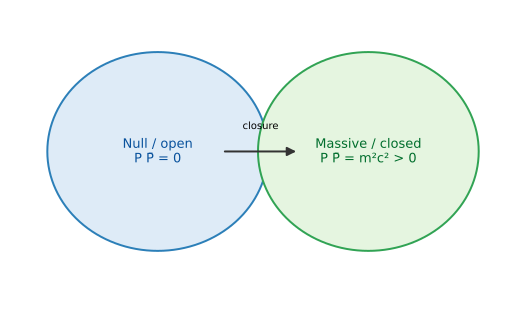
\includegraphics[width=0.80\textwidth]{../assets/figures/mass-shell-norm.svg}
\caption{Norm interpretation of null/open and massive/closed regimes in terms of $P\bar P$.}
\end{figure}

\section{Interpretation and Discussion}
Interpretive regimes:
\begin{itemize}
  \item $P\bar P=0$: null/open propagation.
  \item $P\bar P>0$: massive/closed invariant norm.
\end{itemize}

The phrase ``light that has closure becomes mass'' is interpretive shorthand for transition from null to positive invariant norm.

Define
\[
\bar\lambda_C=\frac{\hbar}{mc},\qquad k_C=\frac{mc}{\hbar}=\bar\lambda_C^{-1}.
\]
$k_C$ is the bridge variable connecting invariant mass to inverse-length scale for Paper 4.

\section{Interpretive Boundaries}
\begin{itemize}
  \item We do \textbf{not} derive observed particle masses.
  \item We do \textbf{not} replace QFT or the Standard Model.
  \item We do \textbf{not} claim a dynamical mass-generation mechanism in this paper.
  \item We do \textbf{not} claim zeta zeros are particles.
\end{itemize}

\section{Conclusion}
We established mass-shell Perfect Closure as a strict invariant-norm statement: $P\bar P=m^2c^2$. We clarified null/open versus massive/closed distinction and identified $k_C=mc/\hbar$ as the bridge variable for operator coupling in Paper 4.

\section*{References}
\begin{enumerate}
  \item A. Einstein, \emph{Zur Elektrodynamik bewegter Koerper}, 1905.
  \item W. R. Hamilton, \emph{Elements of Quaternions}, 1866.
  \item S. L. Adler, \emph{Quaternionic Quantum Mechanics and Quantum Fields}, Oxford Univ. Press, 1995.
\end{enumerate}

\end{document}
